\chapter{Proposition de dataset}
\label{chap:proposition_modele}

Ce chapitre va explorer la création d'un dataset annoté d'images.

\localtableofcontents

\newpage

% -----------------------------------------------------------------------------
% -----------------------------------------------------------------------------
\section{Introduction}
L'examen des datasets disponibles (Section \ref{sec:dataset_disponible}) révèle une carence majeure : seul le dataset RID propose des annotations pour les espaces libres sur toitures. Ce dataset présente toutefois des limitations importantes, avec des images concentrées sur un contexte architectural spécifique (rural allemand) et des performances dégradées lors des tests sur d'autres typologies de bâtiments, comme le démontrent les essais sur le milieu urbain bruxellois.

La création d'un dataset pour une tâche telle que la segmentation sémantique d'image est une tâche laborieuse et chronophage. La première section de chapitre va explorer certaines pistes envisagées qui n'ont finalement pas été retenues. Cette section permet de justifier la nécessité de créer un tel jeu de données annoté.

La deuxième section explore la création du dataset et finalement une troisième section va permettre de faire une synthèse en guise de conclusion de ce chapitre.

% -----------------------------------------------------------------------------
% -----------------------------------------------------------------------------
\section{Méthodologie}
Cette section détaille comment le dataset a été réalisé. Les étapes importantes sont l'obtention des données, le nettoyage, la préparation, la vérification et annotation des données.
\subsection{Données utilisées}
Les données utilisées proviennent de \acrshort{sitg}:
\begin{itemize}
    \item Données vectorielles
    \begin{itemize}
        \item Bâtiments hors-sol ``CAD\_BATIMENT\_HORSOL'' \cite{sitg_batiments_nodate}
        \item Toits des bâtiments ``CAD\_BATIMENTS\_HORSOL\_TOIT'' \cite{sitg_toits_nodate}
        \item Superstructures des toits des bâtiments ``CAD\_BATIMENT\_HORSOL\_TOIT\_SP'' \cite{sitg_superstructures_nodate}
        \item Communes genevoises ``CAD\_COMMUNE'' \cite{sitg_communes_nodate}
    \end{itemize}
    \item Données raster (images)
    \begin{itemize}
        \item Orthophotos 2019 \cite{sitg_orthophotos_nodate}
    \end{itemize}
\end{itemize}
\subsubsection{Données vectorielles}
Les données vectorielles sont en format GPKG \cite{noauthor_ogc_nodate}, ce format est assez commun dans le monde de la géomatique.
\todo[inline]{Ajouter ici le lien correct à l'annexe des données vectorielles}
\paragraph{Bâtiments hors-sol}
La couche vectorielle ``CAD\_BATIMENTS\_HORSOL'' recense tous les bâtiments du Canton de Genève qui sont bien ancrés au sol. Cette couche n'inclus pas les bâtiments qui sont sous-terrains. La Figure \ref{fig:dataset_methodo_01_batiment_horsol} permet d'observer ces polygones qui représentent les bâtiments en orange. Seulement le contour de la toiture est représenté.
\begin{figure}[H]
    \centering
    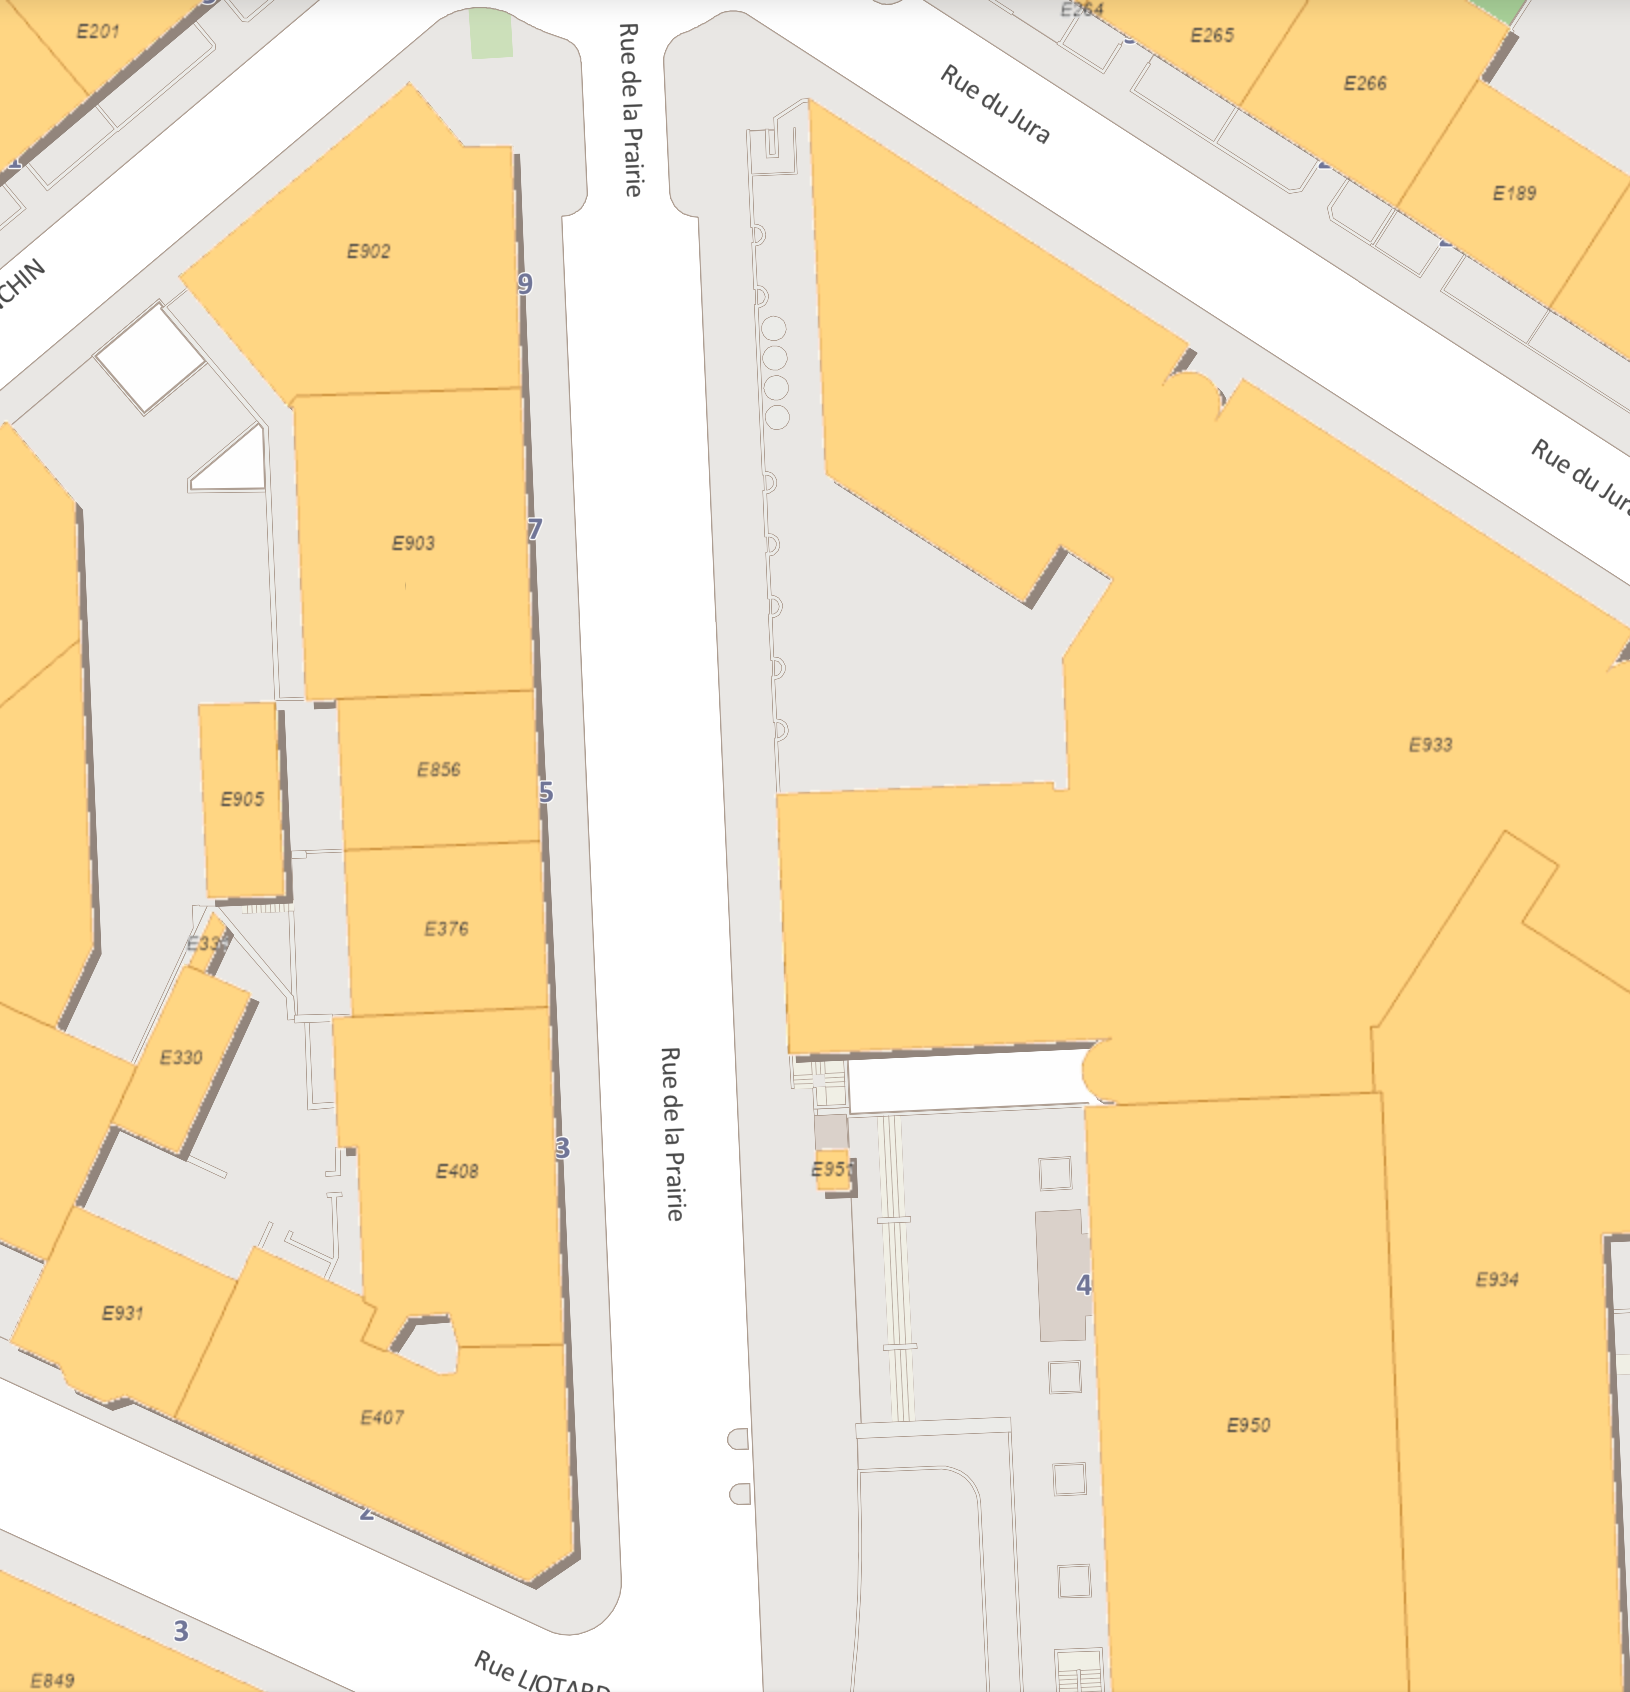
\includegraphics[width=1\linewidth]{02-main//figures/dataset_methodo_01_batiment_horsol.png}
    \caption{Couche vectorielle bâtiments hors-sol.}
    \label{fig:dataset_methodo_01_batiment_horsol}
\end{figure}
Cette couche vectorielle est enrichie de données tabulaires (Figure \ref{fig:dataset_methodo_02_batiment_horsol_donnees}) associées à chacun des polygones.
\begin{figure}[H]
    \centering
    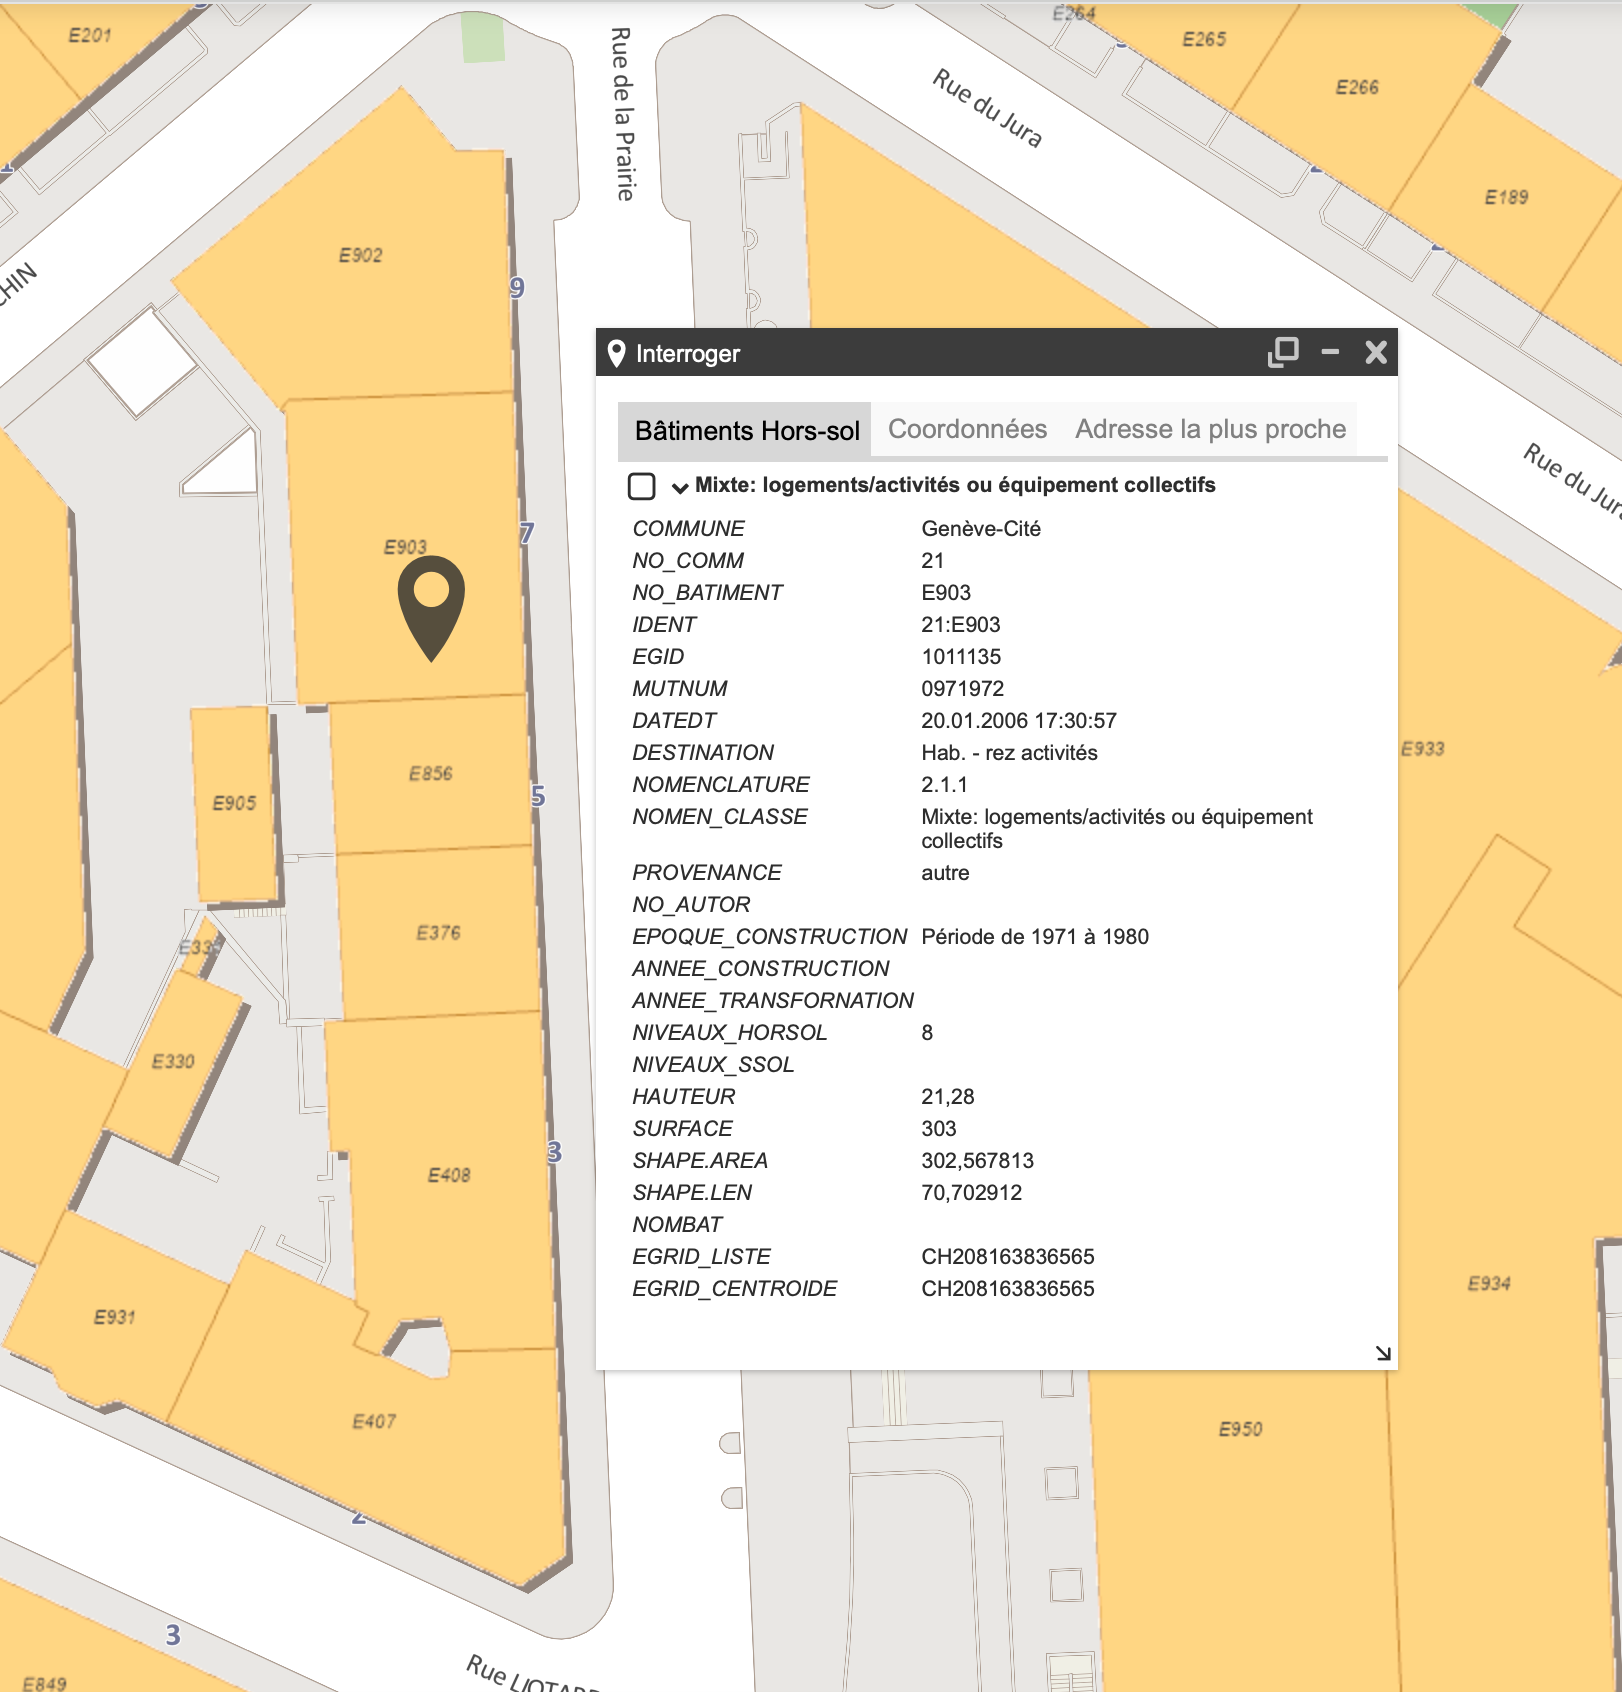
\includegraphics[width=1\linewidth]{02-main//figures/dataset_methodo_02_batiment_horsol_donnees.png}
    \caption{Exemple de données tabulaire associée a un bâtiment (polygone)}
    \label{fig:dataset_methodo_02_batiment_horsol_donnees}
\end{figure}
Les données intéressantes sont l'``EGID'' et ``NOMEN\_CLASSE''. L'EGID est un identifiant unique pour tous les bâtiments en Suisse


% -----------------------------------------------------------------------------
% -----------------------------------------------------------------------------
\section{Pistes explorées non retenues}
\subsection{Introduction}
Cette section va permettre de synthétiser les approches essayées mais qui n'ont pas été retenues. Ce travail exploratoire est nécessaire mais il peut être difficile à valoriser à sa juste valeur.

La première sous-section va explorer la classification des données des toitures et l'utilisation de segment anything model, ensuite la deuxième va explorer les possibilités d'utilisation du dataset RID.

\subsection{Classification}
\subsubsection{Hypothèse}
\acrshort{sitg} met à disposition des données concernant les toitures mais aussi les superstructures présentes sur ces toitures. Une approche naïve serait d'estimer que les toitures qui ne disposent d'aucune superstructure dans leur toiture sont a priori libres. Les toitures restantes avec une superstructures sont ensuite segmentées à l'aide de segment anything model (SAM).

\subsubsection{Données}
Les données utilisées proviennent de \acrshort{sitg}:
\begin{itemize}
    \item Emprise des toitures au sol ``CAD\_BATIMENTS\_HORSOL\_TOIT'' \cite{sitg_toits_nodate}
    \item Superstructures des toits des bâtiments ``CAD\_BATIMENT\_HORSOL\_TOIT\_SP'' \cite{sitg_superstructures_nodate}
    \item Pourcentage des besoins de chauffage couverts
\end{itemize}







